\documentclass[11pt]{article}
\usepackage{amsmath,amssymb,graphicx,xcolor,tikz}
\usetikzlibrary{arrows.meta,calc,positioning}
\newcommand{\M}{\mathcal M}
\newcommand{\R}{\mathbb R}
\newcommand{\T}{\mathsf T}
\newcommand{\Wwin}{\mathcal W}
\newcommand{\Hscore}{\mathcal H}
\DeclareMathOperator{\reach}{reach}
% Numbering in the submitted manuscript.
\makeatletter
\newlabel{prop:pilot}{{3.1}{}}
\newlabel{prop:step}{{3.2}{}}
\newlabel{prop:finite}{{3.3}{}}
\newlabel{prop:readout}{{3.4}{}}
\newlabel{thm:isolated-rank}{{3.5}{}}
\makeatother
\pagestyle{empty}
\begin{document}
\setbox0=\hbox\bgroup
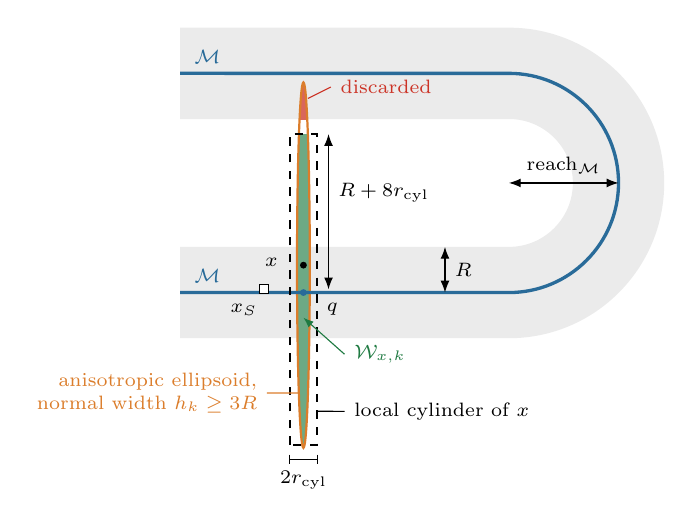
\begin{tikzpicture}[scale=0.58, font=\scriptsize]
  \definecolor{lcblue}{rgb}{0.16,0.42,0.60}
  \definecolor{lcorange}{rgb}{0.86,0.49,0.17}
  \definecolor{lcred}{rgb}{0.80,0.20,0.15}
  \definecolor{lcgreen}{rgb}{0.12,0.48,0.26}
  % tube of radius R=1 around a curve whose bend has radius 2.4 (the reach)
  \fill[black!8] (-4.2,-1) -- (3,-1) arc[start angle=-90, end angle=90, radius=3.4]
     -- (-4.2,5.8) -- (-4.2,3.8) -- (3,3.8) arc[start angle=90, end angle=-90, radius=1.4]
     -- (-4.2,1) -- cycle;
  % Anisotropic ellipsoid: normal half-width 4 > reach; its intersection
  % with the local cylinder is the pooling neighborhood, also outside the tube.
  \begin{scope}
    \clip (-1.8,-3.33) rectangle (-1.2,3.47);
    \fill[lcgreen!65] (-1.5,0.6) ellipse [x radius=0.14, y radius=4.0];
  \end{scope}
  % Its intersection with the distant part of the predictor tube is discarded.
  \begin{scope}
    \clip (-4.2,3.8) rectangle (3,5.8);
    \fill[lcred!75] (-1.5,0.6) ellipse [x radius=0.14, y radius=4.0];
  \end{scope}
  \draw[lcorange, thick] (-1.5,0.6) ellipse [x radius=0.14, y radius=4.0];
  % the manifold
  \draw[lcblue, very thick] (-4.2,0) -- (3,0) arc[start angle=-90, end angle=90, radius=2.4] -- (-4.2,4.8);
  \node[lcblue, above] at (-3.6,0) {$\M$};
  \node[lcblue, above] at (-3.6,4.8) {$\M$};
  % local cylinder: half-width r_cyl=0.3 about x, half-height R+8r_cyl=3.4 about the plane through x_S
  \draw[dashed, thick] (-1.8,-3.33) rectangle (-1.2,3.47);
  % points
  \fill (-1.5,0.6) circle [radius=0.075];
  \node[anchor=east] at (-1.85,0.66) {$x$};
  \fill[lcblue] (-1.5,0) circle [radius=0.075];
  \node[anchor=north west] at (-1.2,-0.02) {$q$};
  \draw[fill=white] (-2.47,-0.03) rectangle (-2.27,0.17);
  \node[anchor=north east] at (-2.3,-0.05) {$x_S$};
  % dimensions
  \draw (-1.8,-3.55) -- (-1.8,-3.75) (-1.2,-3.55) -- (-1.2,-3.75) (-1.8,-3.65) -- (-1.2,-3.65);
  \node[below] at (-1.5,-3.7) {$2r_{\rm cyl}$};
  \draw[<->, >={Latex[length=1.5mm]}] (-0.95,0.07) -- (-0.95,3.47)
     node[pos=0.62, right] {$R+8r_{\rm cyl}$};
  \draw[<->, >={Latex[length=1.5mm]}] (1.6,0) -- (1.6,1) node[midway, right] {$R$};
  \draw[<->, >={Latex[length=1.5mm]}] (3,2.4) -- (5.4,2.4) node[midway, above] {$\reach_\M$};
  % labels
  \node[lcorange, anchor=east, align=right] (nb) at (-2.3,-2.2) {anisotropic ellipsoid,\\normal width $h_k\ge3R$};
  \draw[lcorange, thin] (nb.east) -- (-1.62,-2.2);
  \node[lcgreen, anchor=west] (pool) at (-0.6,-1.35) {$\Wwin_{x,k}$};
  \draw[lcgreen, thin, -{Latex[length=1.3mm]}] (pool.west) -- (-1.5,-0.55);
  \node[anchor=west] (lc) at (-0.6,-2.6) {local cylinder of $x$};
  \draw[thin] (lc.west) -- (-1.2,-2.6);
  \node[lcred, anchor=west] (dc) at (-0.9,4.5) {discarded};
  \draw[lcred, thin] (dc.west) -- (-1.4,4.25);
\end{tikzpicture}
\egroup
\pdfpagewidth=\dimexpr\wd0+4pt\relax
\pdfpageheight=\dimexpr\ht0+\dp0+4pt\relax
\hoffset=-1in \voffset=-1in
\shipout\vbox{\kern2pt\hbox{\kern2pt\box0}}
\end{document}
